\section{An\'alisis te\'orico del circuito}



	\subsection{Polarizaci\'on}
		A continuaci\'on se muestra una imagen del modelo del circuito considerando que los capacitores representan circuitos abiertos, ya que en este caso se trabaja con la señal continua, el mismo se esquematiza con el cálculo del equivalente de thevenin ya realizado entre el nodo de base y tierra.\\
		\begin{figure}[H]
			\centering
			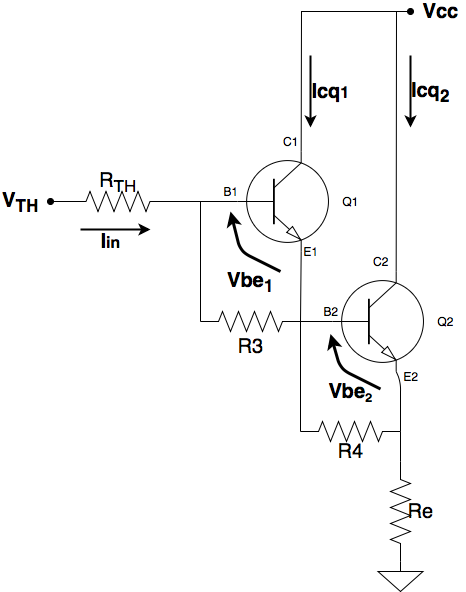
\includegraphics[scale=0.4]{./Imagenes/polarizacion.png} \\
			\caption{Circuito equivalente para el an\'alisis de polarizaci\'on.}
			\label{polarizacion}
		\end{figure}

En la figura \ref{polarizacion} se puede ver el circuito de polarización del transistor. Los valores utilizados para los cálculos fueron los comerciales de los componentes que se utilizaron luego para las mediciones, que fueron previamente elegidos en base a las simulaciones realizadas, con la finalizada de lograr un resultado óptimo. De esta forma, los valores de los componentes utilizados se listan en la tabla \ref{tabla_valores}.

\begin{table}[H]
\centering
\caption{Valores de los componentes utilizados}
\begin{tabular}{ll}
\hline
\multicolumn{2}{l}{\begin{tabular}[c]{@{}l@{}}Parámetros\\   del circuito\end{tabular}} \\ \hline
Vcc                                     & 15,00E+00                                     \\
R1                                      & 100,00E+03                                    \\
R2                                      & 330,00E+03                                    \\
Rs                                      & 10,00E+03                                     \\
R4                                      & 10,00E+03                                     \\
RE                                      & 4,70E+03                                      \\
RL                                      & 1,00E+03                                   
\end{tabular}
\label{tabla_valores}  
\end{table}


Si se realiza el modelo equivalente de thevenin para los nodos de base y tierra, se podrán obtener las siguientes expresiones.\\

		$
		\begin{cases}
		&V_{TH} = \frac{R_2}{R_1 + R_2} V_{CC}\\ \\
		&R_{TH} = R_1 // R_2 
		\end{cases}
		\label{Thevenin}
		$\\

A continuación se muestran las ecuaciones correspondientes al análisis de la malla de entrada, el transistor 2, el transistor 1 y el nodo conectado a la base del 2do transistor\\

		$
		\begin{cases}
		ME) \, \, V_{th}-I_{B1}R_{th}-V_{BEon_{1}}-V_{BEon_{2}}-R_{e}(I_{E_{2}}+I_{R_{4}})=0 \\  \\
		Q_{2}) I_{E_{2}}=I_{B_{2}}(\beta_{2}+1)\\ \\
		Q_{1}) \, \, I_{E_{1}} = I_{B_{1}}(\beta_{1}+1)\\ \\
		Nodo) \, \, I_{B_{2}} = I_{E_{1}} - \frac{V_{BEon_{2}}}{R_{4}}
		\end{cases}
		$\\

Con ellas ecuaciones, resolviendo se puede llegar a las siguientes expresiones para las corrientes de colector de ambos transistores.\\

		$
		\begin{cases}
		I_{cq_{1}}=\frac{V_{th}-V_{BEon_{1}}-V_{BEon_{2}}\left(1-\frac{R_{e}\beta_{2}}{R_{4}}\right)}{\frac{R_{th}}{\beta_{1}}+R_{e}\beta_{2}}\\ \\
		I_{cq_{2}}=V_{th}\frac{1}{\frac{R_{th}}{\beta_{1}\beta_{2}}+R_{e}\frac{\beta_{2}+1}{\beta_{2}}}-V_{BEon_{1}}\frac{1}{\frac{R_{th}}{\beta_{2}}+R_{e}\beta_{1}}-V_{BEon_{2}}\left(\frac{\beta_{2}}{R_{4}}+\frac{\left(1-\frac{R_{e}\beta_{2}}{R_{4}}\right)\cdot(\beta_{1}+1)}{\frac{R_{th}}{\beta_{2}}+R_{e}\beta_{1}} \right)
		\end{cases}
		$\\

Así recorriendo la malla de salida se puede ver que se obtienen las siguientes relaciones.\\

		$
		\begin{cases}
		V_{CEQ_{1}}=V_{CC}-V_{BEon_{2}}\left(1+\frac{R_{e}}{R_{4}}\right)-R_{e}I_{CQ_{2}}\\ \\
		V_{CEQ_{2}}=V_{CC}-V_{BEon_{2}}\frac{R_{e}}{R_{4}}-R_{e}I_{CQ_{2}}
		\end{cases}
		$\\
	
Y si se reemplaza por los valores utilizados, nombrados anteriormente y considerando en ambos transistores la $V_{BEon}=0.7(V)$, con sus HFE de valor 47 y 90 respectivamente, se pueden hallar los valores de $I_{cq_{1}}$, $I_{cq_{2}}$, $V_{CEQ_{1}}$ y $V_{CEQ_{2}}$, los mismos se encuentran detallados en la tabla \ref{tabla_valores_polarizacion}.

\begin{table}[H]
\centering
\caption{Valores hallados para las componentes de polarizacion.}
\begin{tabular}{ll}
\multicolumn{2}{l}{Polarización} \\ \hline
ICQ1          & 93,54E-06        \\
ICQ2         & 2,12E-03         \\
VCEQ1         & 4,01E+00         \\
VCEQ2         & 4,71E+00        
\end{tabular}
\label{tabla_valores_polarizacion}  
\end{table}

\todo{tabla con icq y vce}


	\subsection{Modelo incremental}
	
	Se tiene que para cada transistor los estimadores tomados son los que se detallan a continuación.


		\begin{equation}
			\begin{cases}
			\widehat{r_{e}}=\frac{V_{T}}{I_{CQ}}\\
			\widehat{h_{ie}}=(\beta_{i}+1)R_{e_{i}}\\	
			\widehat{gm}=\frac{1}{R_{E}}
			\end{cases}
			\label{mod_inc_ecs}
		\end{equation}
	
	De esta forma, para el transistor $Q1$ se emplean las ecuaciones \ref{mod_inc_ecs} reemplazando i por 1, mientras que para el transistor $Q2$ se reemplaza i por 2. Así se obtienen los siguientes valores:
	
	\todo{COMPLETAR TABLA de estimadores}
	\begin{table}[h!]
		\centering
		\begin{tabular}{c c c}%
			\bfseries Estimadores & Q1 & Q2 \\ \hline
			$\widehat{g}_m$ &  & \\
			$\widehat{h}_{ie}$ &  & \\
			$\widehat{r}_{e}$&  & \\
			\hline
		\end{tabular}
		\caption{Estimadores correspondientes al modelo incremental, para los transistores Q1 y Q2.}
		\label{avolf}
	\end{table}
	
	\subsection{Circuito incremental}
	
		
		\begin{figure}[H]
			\centering
			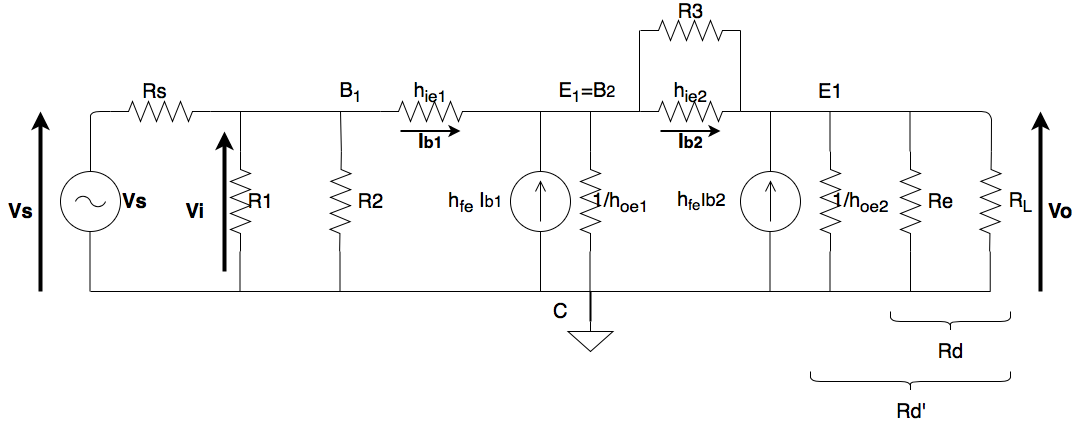
\includegraphics[scale=0.4]{./Imagenes/circ_incremental.png} \\
			\caption{Circuito equivalente para el an\'alisis del circuito incremental.}
			\label{circ_incremental}
		\end{figure}

En la tabla de abajo se muestran los valores utilizados y calculados en esta sección, que permitirán luego conocer los valores deseados, como ser las ganancias de tensión y corriente.

\begin{table}[H]
\centering
\begin{tabular}{ll}
\multicolumn{2}{l}{Modelo incremental} \\ \hline
VT              & 2,60E-02             \\
hfe1            & 47,00E+00            \\
hfe2            & 90,00E+00            \\
hie1            & 13,34E+03            \\
hie2            & 1,12E+03             \\
\end{tabular}
\label{tabla valores} 
\end{table}

A continuacion se muestran las ecuaciones que rigen las reducciones del circuito para facilitar su análisis, las mismas incluyen paralelos de resisitencias y pasaje a nivel de corriente. \\

		$
		\begin{cases}
		hfe_{2}^{*}=hfe_{2}\frac{R_{4}}{R_{4}+hie_{2}} \\
		hie_{2}^{*}=hie_{2}//R_{4} \\
		R_{d}=R_{e}//R_{2}
		\end{cases}
		\label{mod_inc_ecs}
		$ \\

De esta manera, reemplazando por los valores correspondientes se obtendrían los valores mostrados en la tabla siguiente.

\begin{table}[H]
\centering
\begin{tabular}{ll}
\multicolumn{2}{l}{Simplificaciones} \\ \hline
hfe2*          & 80,96E+00           \\
Rd             & 824,56E+00          \\
hie2*          & 1,00E+03           
\end{tabular}
\end{table}

A partir del circuito y de los caálculos anteriores, se puede ver que las expresiones para las impedancias que se ven a la entrada del primer transistor, del amplificador y del sistema se ven representadas por las ecuaciones que se muestran a continuación. \\

		$
		\begin{cases}	
		R_{i}=hie_{1}+(hfe_{1}+1)hie_{2}^{*}+(hfe_{2}^{*}+1)(hfe_{1}+1)R_{d} \\
		R_{ia}=R_{i} // R_{th} \\
		R_{is}=R_{s}+R_{ia}
		\end{cases}
		\label{mod_inc_ecs}
		$\\

De donde reemplanzando por los valores de la tabla \ref{tabla valores} se pueden obtener los siguientes valores

\begin{table}[H]
\centering
\begin{tabular}{ll}
\multicolumn{2}{l}{\begin{tabular}[c]{@{}l@{}}Impedancias\\   de entrada\end{tabular}} \\ \hline
Ri                                      & 3,31E+06                                     \\
Ria                                     & 75,00E+03                                    \\
Ris                                     & 85,00E+03                                   
\end{tabular}
\end{table}

A continuación se muestran dos expresiones halladas que servirán de base para luego facilitar el cálculo de la ganancia del sistema.\\

		$
		\begin{cases}	
		\frac{V_{o}}{ib_{2}}=R_{d}(hfe_{2}^{*}+1) \\
		\frac{V_{i}}{V_{s}}=\frac{R_{ia}}{R_{ia}+R_{s}}
		\end{cases}
		\label{mod_inc_ecs}
		$\\

Así la ecuación de la ganancia en tensión del sistema se puede expresar de la siguiente forma. \\

	\begin{equation}	
		\Delta _{vs}=\frac{V_{o}}{V_{s}}=\frac{V_{o}}{ib_{2}}\cdot\frac{ib_{2}}{ib_{1}}\cdot\frac{ib_{1}}{V_{i}}\cdot\frac{V_{i}}{V_{s}}=R_{d}(hfe_{2}^{*}+1)(hfe_{1}+1)\frac{1}{R_{i}}\frac{Ria}{Ria+Rs}
		\label{mod_inc_ecs}
	\end{equation}

De esta manera reemplazando por los valores de los componentes de la ecuación se puede llegar a la siguiente tabla.

\begin{table}[H]
\centering
\begin{tabular}{ll}
\multicolumn{2}{l}{\begin{tabular}[c]{@{}l@{}}Ganancias\\   de tension\end{tabular}} \\ \hline
Av                                       & 0,981                                     \\
Avs                                      & 0,866                                    
\end{tabular}
\end{table}


A la ganancia de corriente se la puede expresar como \\

	\begin{equation}	
		\Delta _{i}=\frac{I_{Rd}}{ib_{1}}=(hfe_{2}^{*}+1)(hfe_{1}+1)
		\label{mod_inc_ecs}
	\end{equation}

	\begin{equation}	
	\Delta_{is}=\frac{I_{Rd}}{I_{Rs}}\cdot\frac{I_{b_{1}}}{I_{Rs}}=\Delta_{i}\frac{R_{th}}{R_{th}+R_{i}}
	\label{mod_inc_ecs}
	\end{equation}

	\begin{equation}	
		\Delta_{is}^{\, \, \,'}=\frac{I_{Rl}}{I_{Rs}}=\frac{I_{Rl}}{I_{Rd}}\cdot\frac{I_{Rd}}{I_{Rs}}=\frac{R_{e}}{R_{e}+R_{2}}\Delta_{is}
		\label{mod_inc_ecs}
	\end{equation}

Donde $\Delta_{i}$ es la ganancia de corriente, $\Delta_{is}$ es la ganancia de corriente del sistema y $\Delta_{is}^{\, \, \,'}$ es la ganancia de corriente del sistema sobre la carga, los valores de las mismas se muestran en la siguiente tabla.

\begin{table}[H]
\centering
\begin{tabular}{ll}
\multicolumn{2}{l}{\begin{tabular}[c]{@{}l@{}}Ganancias\\   de corriente\end{tabular}} \\ \hline
Ai                                       & 3934,08                                     \\
Ais                                      & 89,27                                       \\
Ais'                                     & 73,61                                      
\end{tabular}
\end{table}

Las siguientes ecuaciones son las que permiten hallar la resistencia ro,  la cual es la resistencia de salida del transistor.\\

$
		\begin{cases}	
		I_{op}=I_{B1}(hfe_{1}+1)(hfe_{2}^{*}+1)\\
		V_{op}=I_{B1}(R_{s}//R_{th}+h_{ie1})+(hfe_{1}+1)hie_{2}^{*}I_{B2} \\
		r_{o}=\frac{V_{op}}{I_{op}}=\frac{R_{s}//R_{th}+hie1+(hfe1+1)hie_{2}^{*}}{(hfe_{1}+1)(hfe_{2}^{*}+1)}\\
		r_{oa}=R_{e}//r_{o}\\
		r_{os}=r_{oa}//Rl
		\end{cases}
		\label{mod_inc_ecs}
		$\\

De esta manera, y reemplazando por los valores de las variables involucadas en la ecuación, se puede llegar a la siguiente tabla con los valores de las resistencias de salida.

\begin{table}[H]
\centering
\begin{tabular}{ll}
\multicolumn{2}{l}{Impedancias de salida} \\ \hline
ro                & 15346,62              \\
roa               & 3598,07               \\
ros               & 782,52               
\end{tabular}
\end{table}

\section{Diseño del circuito}